\documentclass[
    ngerman,
    color=3b,
    % dark_mode,
    load_common, % Loads a list of commonly used Packages
    summary,
    boxarc,
    % manual_term,
    % solution=true,
]{tuda_summary} 
% Import all Packages from Main Preamble with relative Path
% \subimport*{../../}{preamble}
% Get Labels from Main Document using the xr-hyper Package
\externaldocument{../../AuD-Zusammenfassung-2020}
% Set Graphics Path, so pictures load correctly
\graphicspath{{../../}}


\begin{document}
\section{Randomized Data Structures}\label{Randomized Data Structures}\index{Randomized Data Structures}
\subsection{Skip Lists}\label{Skip Lists}\index{Skip Lists}
\begin{idea}[skip Lists]\mbox{}
    \begin{itemize}
        \item Einfügen von "`Express-Liste"'\index{Express-Liste} mit einigen Elementen
        \item Beginne mit Suche in der Express-Liste mit weniger Elementen
        \item Falls das suchende Element kleiner als nächstes Element in Express-Liste $\Rightarrow$ weiter nach rechts
        \item Falls nicht $\Rightarrow$ Eine Stufe nach unten wandern und dort weiter suchen
    \end{itemize}
\end{idea}

\begin{description}[itemsep=1em]
    \item [Mögliche Verbesserung] \begin{itemize}
              \item Zusätzliche Stufen an Express-Listen
          \end{itemize}
    \item [Anwendung]
          \begin{itemize}
              \item Gut für parallele Verarbeitung z.B. Multicore-Systeme (Einfügen und Löschen)
              \item Dafür logarithmische Laufzeit nur im Durchschnitt
          \end{itemize}
    \item [Auswahl von Elementen]
          \begin{itemize}
              \item Abhängig von einer gewählten Wahrscheinlichkeit $p$
              \item Element kommt mit Wahrscheinlichkeit $p$ in übergeordnete Liste
              \item Höhe: $h = O(log_{\frac{1}{p}}n)$
              \item Anzahl Elemente: $n \Rightarrow pn \Rightarrow p^2n \Rightarrow ...$ (unten nach oben)
          \end{itemize}
\end{description}

\paragraph{Implementierung}\mbox{}\\
\begin{minipage}{.60\textwidth-2.22166pt}
    \centering
    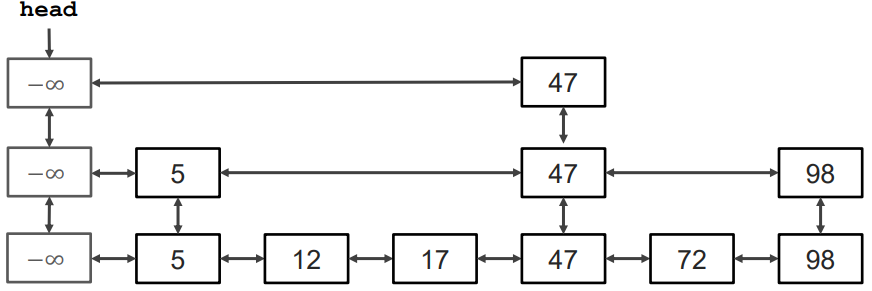
\includegraphics[width=\textwidth]{pictures/skiplistImplement1.PNG}\\
    \captionof{figure}{Beispiel Skip List}
\end{minipage}
\begin{minipage}{.4\textwidth}
    \centering
    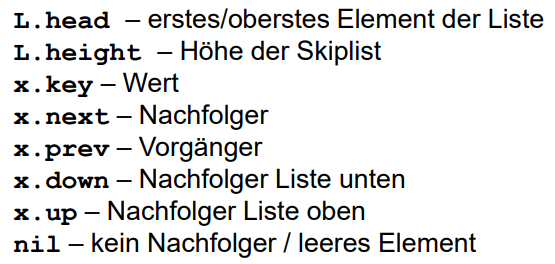
\includegraphics[width=\textwidth]{pictures/skiplistImplement2.PNG}
\end{minipage}

\clearpage
\paragraph{Suche}\mbox{}\\
Laufzeit ist von Expresslisten abhängig
%\begin{noindent}
\begin{codeBlock}[autogobble]{title={search(L, k)}}
current = L.head;
WHILE current != nil DO
    IF current.key == k THEN 
        return current;
    IF current.next != nil AND current.next.key <= k THEN
        current = current.next;
    ELSE
        current = current.down;
return nil;
\end{codeBlock}
%\end{noindent}

\begin{figure}[h]
    \centering
    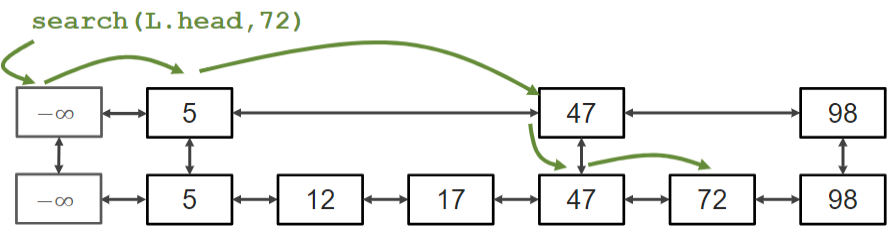
\includegraphics[width=12cm]{pictures/skiplistSuche.PNG}
    \caption{Beispiel Suche in einer Skip List}
\end{figure}
\paragraph{Einfügen}
\begin{itemize}
    \item Füge auf unterster Ebene ein
    \item Evtl. auf höheren Ebenen mit zufälliger Wahl mithilfe von $p$ auf jeder Ebene
    \item falls ein Element nicht auf die nächst höhere Ebene gelangt, gelangt es auch nicht auf andere höhere Ebenen (Abbruch des Auswahlprozesses)
\end{itemize}

\paragraph{Löschen}
\begin{itemize}
    \item Entferne Vorkommen des Elements aus allen Ebenen
\end{itemize}

\paragraph{Laufzeiten}
\begin{description}[leftmargin=2cm]
    \item [Einfügen] $\Theta(log_{\frac{1}{p}}n)$
    \item [Löschen] $\Theta(log_{\frac{1}{p}}n)$
    \item [Suchen] $\Theta(log_{\frac{1}{p}}n)$
\end{description}
\begin{itemize}
    \item $O$-Notation versteckt konstanten Faktor $\frac{1}{p}$
    \item Speicherbedarf im Durchschnitt: $\frac{n}{1-p}$
\end{itemize}
\clearpage
\subsection{Hashtables}\label{Hashtables}\index{Hashtables}
\mbox{}\vspace{-2em}
\begin{wrapfigure}[1]{r}{0.4\textwidth}
    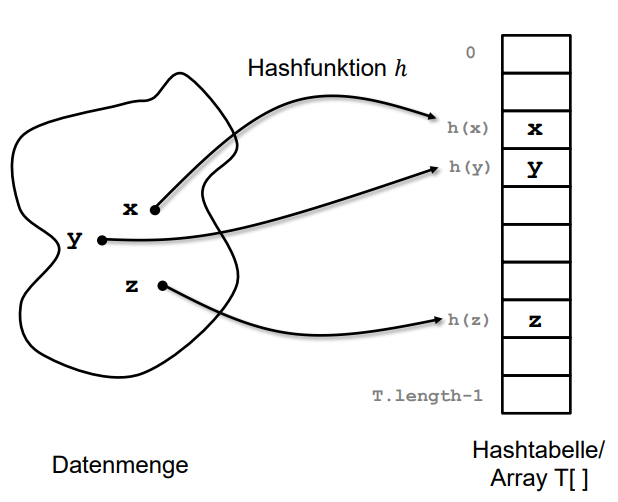
\includegraphics[width=0.4\textwidth]{pictures/hashtableIdee.PNG}
    \captionof{figure}{Beispiel Hashfunktion}
\end{wrapfigure}
\begin{idea}[Hashtable]\mbox{}
    \begin{itemize}
        \item Hashfunktion sollte gut verteilen
        \item $h(x)$ sollte uniform sein
        \item Unabhängig im Intervall $[0, T.length-1]$ verteilt
        \item Einfügen mit konstant vielen Array-Operationen
        \item Kollisionsauflösung z.B. mithilfe von LinkedLists
        \item Neue Elemente werden vorne angefügt
        \item Konstante Anzahl an Array-Operationen
        \item Soviele Schritte wie die Liste lang ist
        \item Uniforme Hashfunktion
        \item[] $\Rightarrow$ $\frac{n}{T.length}$ Einträge pro Liste
    \end{itemize}
\end{idea}

\paragraph{Hash-Funktionen}\index{Hash-Funktion}
\begin{description}[itemsep=1em,leftmargin=6cm]
    \item [Universelle Hash-Funktion]\index{Hash-Funktion!universell}
          \begin{itemize}
              \item Wähle zufällige $a,b \in [0, p - 1]$, $p~prim$, $a \neq 0$
              \item $h_{a,b}(x)= ((a \cdot x + b)~mod~p)~mod~T.length$
          \end{itemize}
    \item [Krypthographische Hash-Funktionen]\index{Hash-Funktion!Kryptographisch}%
          \begin{itemize}%
              \item MD5, SHA-1, SHA-2, SHA-3
              \item $h(x) = MD5(x)~mod~T.length$
          \end{itemize}
\end{description}
\begin{wrapfigure}[5]{r}{0.4\textwidth}
    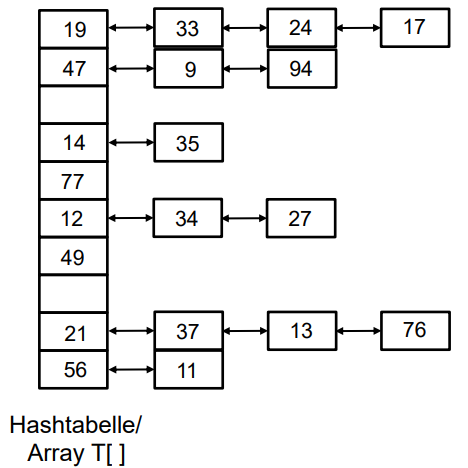
\includegraphics[width=0.4\textwidth]{pictures/hashtableLinkedList.PNG}
    \captionof{figure}{Beispiel Hashtabelle}
\end{wrapfigure}
\paragraph{Hashtables vs. Bäume}
\begin{description}[itemsep=1em,leftmargin=2cm]
    \item [Hashtables]
          \begin{itemize}
              \item nur Suche nach bestimmten Wert möglich
              \item meist grö\ss{}er als zu erwartende Anzahl Einträge
          \end{itemize}
    \item [Bäume]
          \begin{itemize}
              \item schnelles Traversieren zu Nachbarn möglich
              \item Bereichssuche möglich
          \end{itemize}
\end{description}

\paragraph{Laufzeiten}
\begin{description}[leftmargin=2.3cm]
    \item[Einfügen] $\Theta(1)$
    \item[Löschen] $\Theta(1)$
    \item[Suchen] $\Theta(1)$
\end{description}
\begin{itemize}
    \item Für $T.length = n$ ergibt sich konstante Laufzeit
    \item (Im Durchschnitt, beim Einfügen sogar im Worst-Case)
    \item Speicherbedarf i.d.R. höher als n, meist ca. $1,33 \cdot n$
\end{itemize}

\subsection{Bloom-Filter}\label{Bloom-Filter}\index{Bloom-Filter}
\begin{idea}[Bloom-Filter]\mbox{}\\
    Speicherschonende Wörterbucher mit kleinem Fehlerpotenzial
    z.B. Vermeidung von schlechten Passwörtern
    \begin{enumerate}
        \item Abspeichern aller schlechten Passwörter in kompakter Form
        \item Prüfe, ob eingegebenes Passwort im Bloom-Filter
    \end{enumerate}
    z.B. Erkennen von schädlichen Websites (Chrome früher)
\end{idea}

\paragraph{Erstellen}\mbox{}
\begin{itemize}
    \item $n$ Elemente $x_0,...,x_{n-1}$
    \item $m$ Bits-Speicher z.B. als Bit-Array
    \item $k$ gute Hash-Funktionen $H_0,...,H_{k-1}$ mit Bildbereich $0,1,...,m-1$
    \item Empfohlene Wahl: $k = \frac{m}{n} \cdot ln2$ (Fehlerrate von ca. $2^{-k}$)
\end{itemize}
Code:\index{initBloom(X,BF,H)}
%\begin{noindent}
\begin{codeBlock}[autogobble]{title={initBloom(X, BF, H) // H Array of hash functions}}
FOR i = 0 TO BF.length - 1 DO 
    BF[i] = 0;
FOR i = 0 TO X.length - 1 DO
    FOR j = 0 TO H.length - 1 DO
        BF[H[j](X[i])] = 1;
\end{codeBlock}
%\end{noindent}

\begin{enumerate}
    \item Initialisiere Array mit "$0$er-Einträgen
    \item Schreibe für jedes Element in jede Bit-Position $H_0(x_i),...,H_{k-1}(x_i)$ eine 1
\end{enumerate}
\begin{figure}[h]
    \centering
    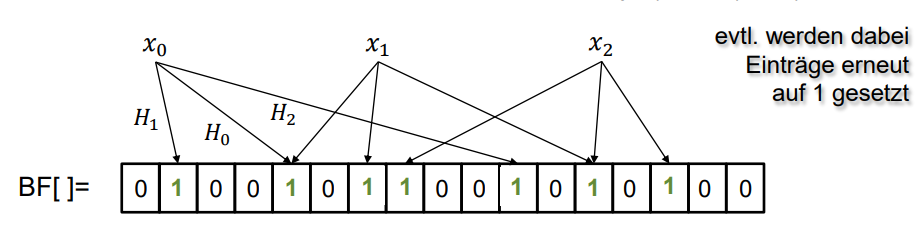
\includegraphics[width=15cm]{pictures/bloomCreate.PNG}
    \caption{Beispiel Bloom Filter}
\end{figure}
\clearpage
\paragraph{Suche}\mbox{}
\index{searchBloom(BF,H,y)}
%\begin{noindent}
\begin{codeBlock}[autogobble]{title={searchBloom(BF, H, y)}}
result = 1;
FOR j = 0 TO H.length - 1 DO
    result = result AND BF[H[j](y)];
return result;
\end{codeBlock}
%\end{noindent}
\begin{itemize}
    \item Gibt an, dass $y$ im Wörterbuch, falls alle $k$ Einträge für $y$ in $BF=1$ sind
\end{itemize}
\begin{figure}[h]
    \centering
    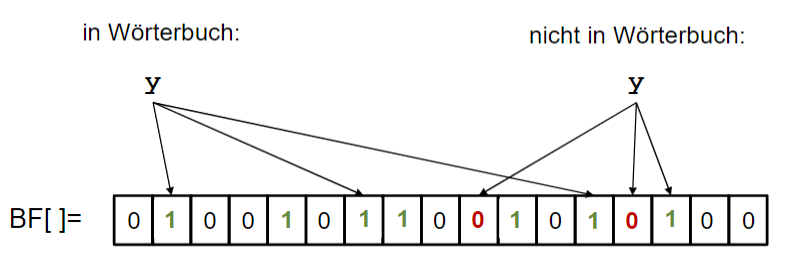
\includegraphics[width=13.5cm]{pictures/bloomSearch.PNG}
    \caption{Beispiel Suche im Bloom Filter}
\end{figure}
\begin{itemize}
    \item Eventuell \string"false positives\string" (1, obwohl $y$ nicht im Wörterbuch)
          \begin{itemize}
              \item Passiert, falls die Einträge vorher von anderen Werten getroffen wurden
              \item Daher gute Hashfunktionen und Filtergrö\ss e nicht zu klein
          \end{itemize}
\end{itemize}
\clearpage
\end{document}
